\part{Sequence of Functions}


\section{Introduction}

In previous courses, we analysed the convergence of sequences of numbers (example: $U_n = \left\{ \frac{1}{4},\frac{1}{9},\frac{1}{16},\ldots \right\} =\sum_{n=1}^{\infty} \frac{1}{n^2} $) with a series of tests. In this course we will be analysing sequences of \emph{functions} $f_n(x)$.\\
An example, is $f_n(x)=\frac{x}{x+n} =\{f_1,f_2,f_3,\ldots\}  =\left\{ \frac{x}{x+1},\frac{x}{x+2},\frac{x}{x+3},\ldots \right\}$.\\

There are 2 ways these sequences can converge: pointwise and uniformly

\begin{figure}[H]
    \centering
    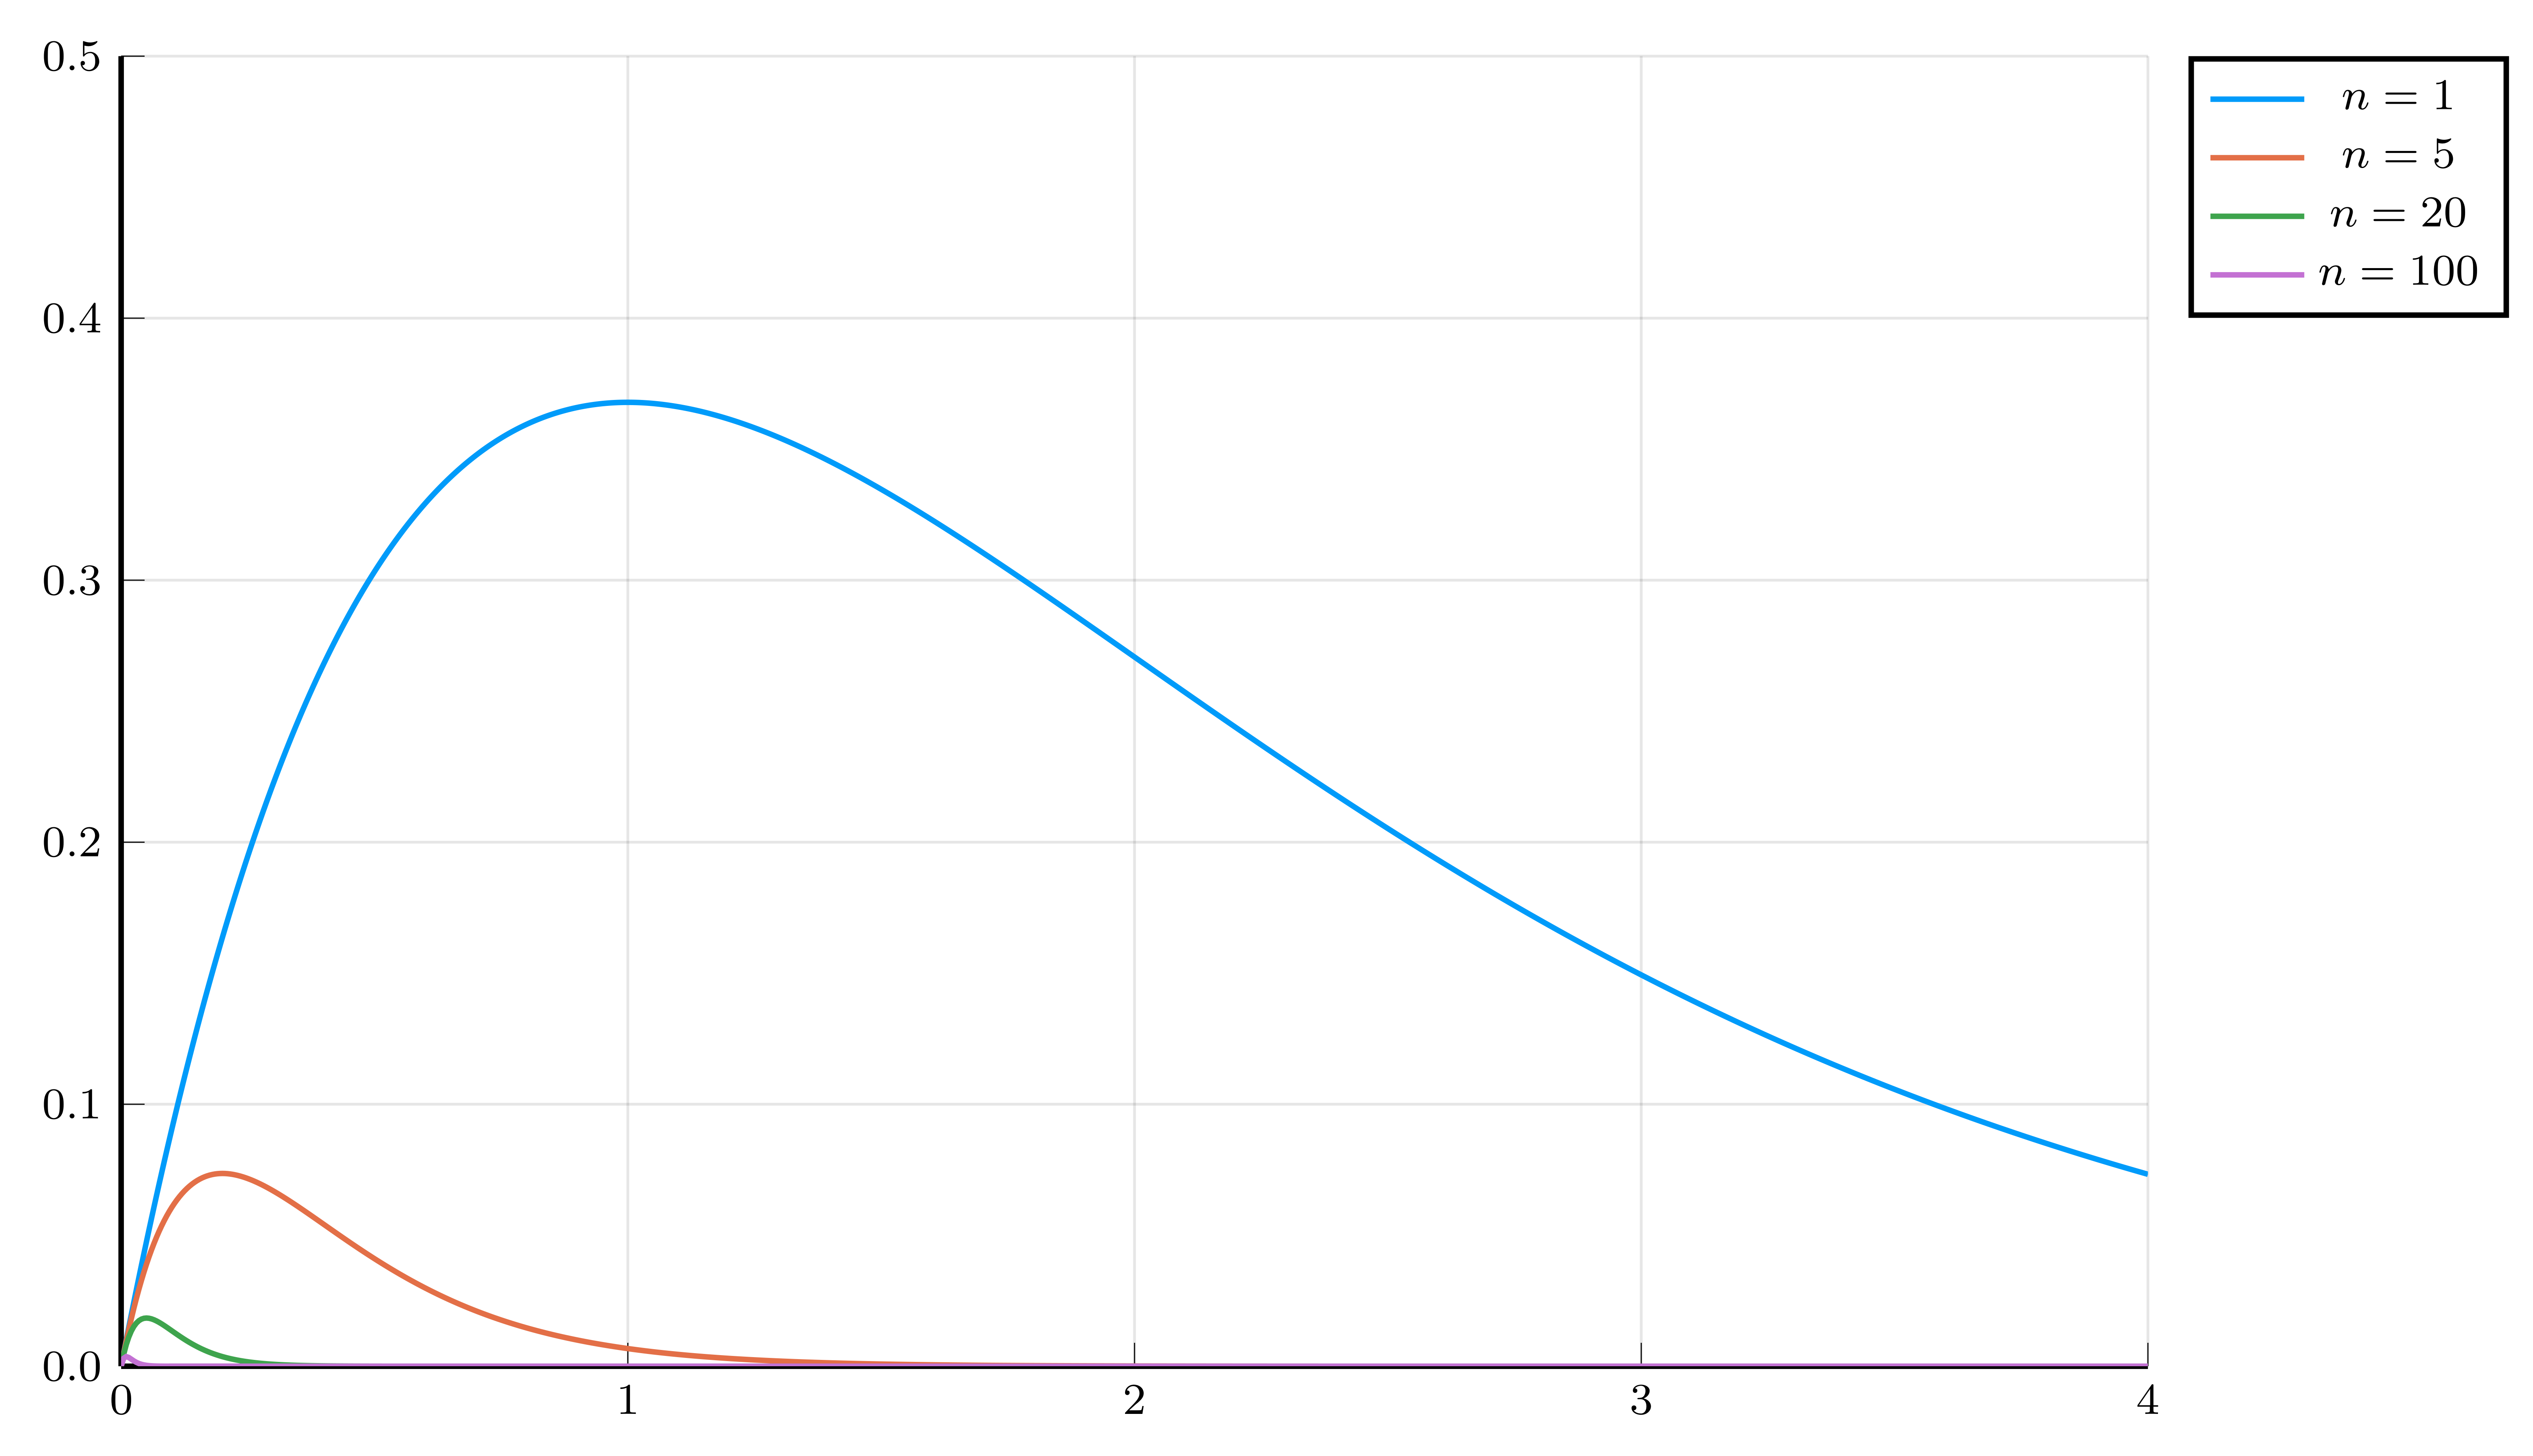
\includegraphics[width=\textwidth]{plot1.png}
    \caption*{Plot of the sequence $f_n(x)=xe^{-nx}$}
    \label{fig:plot}
\end{figure}

\section{Pointwise convergence}

This is a very natural way of proving convergence since all you have to do is fix $f_n$ to a point $x$ then the sequence just becomes an ordinary sequence of numbers, and if they all converge to a number we can define a limit function $f$ and say that they converge to $f$ pointwisely.

\begin{definition}
    We say that a sequence of functions $f_n$ where $f_n:I \to \mathbb{R},I\subset \mathbb{R}$, converges pointwise to function $f:I\to \mathbb{R}$ on the interval $I$ if:
    \[
    \forall x\in I \; \forall \epsilon >0 \; \exists n\in \mathbb{N} \; \forall n\ge \mathbb{N}: \quad \left| f_n(x)-f(x) \right|<\epsilon 
    .\] 
\end{definition}
You either prove convergence using the definition or by doing:
\begin{enumerate}
    \item Let $x=0$ then find $\lim_{n \to \infty} f_n(0)=$ some $f(x)$
    \item Then let $x\neq 0$ and again find $\lim_{n \to \infty} f_n(x)=f(x)$ 
    \item If neither of the results are unbounded $\pm \infty$ then we say $f_n(x)$ is convergent to some $f(x)$
\end{enumerate}

\begin{remark}
    if the result of step 1 is $g(x)$ and step 2 results in $h(x)$ where $g(x)\neq h(x)$ then we define the limit function:
     \[
         f(x)=\begin{cases}g(x)&x=0\\h(x)&x\in ]0,1]\end{cases}
    .\] 
\end{remark}

\section{Uniform convergence}

The idea of uniform convergence is that the sequence always approaches it's limit function as the value of $n$ increases.

\begin{definition}
    We say that a sequence of functions $f_n$ where $f_n:I \to \mathbb{R},I\subset \mathbb{R}$, converges uniformly to function $f:I\to \mathbb{R}$ on the interval $I$ if:
    \[
        \forall \epsilon>0\;\exists N\in\mathbb{N}\;\forall n\ge N\;\forall x\in I: \; \sup_{x\in I} \left| f_n(x)-f(x) \right| <\epsilon
    .\]    
\end{definition}

\begin{remark}
    We can also prove uniform convergence by proving
    \[
        \lim_{n \to \infty}\sup_{x\in I} \left| f_n(x)-f(x) \right|=0 
    .\] 
\end{remark}


Let $f_n$ be a sequence of functions defined on $E\subset \mathbb{R}\}$. We will say that $f_n$ converges pointwise to the function $f$ if for every $\varepsilon>0$ and for every $x\in E, \exists N\in \mathbb{N}$ such that for al $n>N$ $\left|f_n(x) - f(x)\right|<\varepsilon$ we write $\lim_{n \to \infty} f_n(x)=f(x)$.\sn{The integer $N$ depends on $\varepsilon$ and $x$ ;$N(\varepsilon,x)$}
\begin{example}
    Let $f_x(x)=\frac{x}{x+n}$ ;$x\in[0,1]=E$, study the pointwise convergence of $f_n$.\\
    \[
    \lim_{n \to \infty}f_n(x) = 0 
    .\]
    We conclude that $f_n$ converges pointwise to $f(x)=0\quad \forall x\in[0,1]$
\end{example}

\begin{example}
    let $f_n(x)=\frac{nx}{1+nx}$ where $x\in[0,1]=E$. Study the pointwise convergence of $f_n$.
    \begin{itemize}
        \item $x=0$,$x \to +\infty\implies nx\to \infty$. Undetermined form.\\
            $f_n(0)=0\implies\lim_{n \to \infty}f_n(0)=0 $
        \item $x \neq 0$ ($x$ is fixed)\\
            $\lim_{n \to \infty} f_n(x)=\lim_{n \to \infty}\frac{nx}{1+nx}=1 $
    \end{itemize}
    Then $f_n$ converges pointwise to 
    \[
    f(x)=\begin{cases}
        0&\text{if }x=0\\
        1&\text{if }x\in]0,1]
    \end{cases}
    .\] 
\end{example}
\subsection{Second method}
using the definition of the pointwise convergence.
\[
\forall x \in E,\forall \varepsilon>0\; \exists N\in \mathbb{N}/\forall n>N \left|f_n(x)-f(x)\right|<\varepsilon
.\] 
we must find $N$ first for $x=0$ $\left|f_n(0)-f(0)\right|=0-0=0<\varepsilon$ then the choice of $N$ is arbitrary.\\
for $x\neq 0$ \\
\[
\left|f_n(x)-f(x)\right|=\left|\frac{nx}{1+nx}\right|=\left|\frac{1}{nx+1}\right|=\frac{1}{nx+1}<\varepsilon
.\] 
We choose $N$ such that $N\ge \frac{1-\varepsilon}{\varepsilon x}$
\section{Uniform convergence}
\begin{definition}
    Let $f_n$ be a sequence of functions defined on $E\subset \mathbb{R}$. We say that $f_n$ converges uniformly to the limit function $f$ if 
    \[
    \forall \varepsilon>0,\exists N\in \mathbb{N}/\forall n>N \sup_{x\in E}\left|f_n(x)-f(x)\right|<\varepsilon
    .\] 
    $f(x)$ is the limit function $x\in E$.\mn{$N$ depends on only $\varepsilon,N(\varepsilon)$}
\end{definition}
\begin{remark}
    \begin{itemize}
        \item Pointwise convergence means that at every point the sequence of function has its own speed of convergence (that can be very fast at some points and very slow at others)
        \item Uniform convergence means there is an overall speed of convergence
    \end{itemize}
\end{remark}
\begin{example}
     $f_n(x)=\frac{1}{n}x^2$.\\
     $\lim_{n \to \infty}f_n(x)=0$ the sequence $\frac{1}{n}x^2$ CV pointwise to $f(x)=0$ (no overall speed of CV for all points)
\end{example}
\begin{example}
    $g_n(x)=\frac{\sin(nx)}{n}\; ;x\neq 0$\\
   $\lim_{n \to \infty}g_n(x)=0 $ the sequence CV uniform to $g(x)=0$ (there is an overall speed of CV for all points)
\end{example}
\begin{remark}
   To prove the uniform convergence of a sequence of functions $f_n$ defined on $E$ to the limit function, we may prove the pointwise convergence by proving the integer $N$ is independent of $x$ or $\lim_{n \to \infty} \sup \left|f_n(x)-f(x)\right|=0$
\end{remark}

\begin{example}
    Let $f_n(x)=\frac{x}{x+n}\; ; x\in [0,1] \text{ and } n \in \mathbb{N}$.\\
    Study the uniform convergence of $f_n(x)$ to $f(x)=0$ by showing that $N=N(\varepsilon)$.\\\\
    $\lim_{n \to \infty}f_n(x)=0$
    \[
    \left| f_n(x)-f(x) \right| =\frac{x}{x+n}<\varepsilon \implies n>x\left( \frac{1}{\varepsilon}-1 \right) 
    .\] 
    $x\in[0,1]\implies n>\frac{1}{\varepsilon}$, $N>\frac{1}{\varepsilon}\implies N=N(\varepsilon)$ then $f_n$ converges uniformly to $f(x)=0$
\end{example}

\begin{example}
    % TODO table of convergence 
    Let $f_n(x)=\frac{nx}{1+nx}$ defined on $[1,2]$. Show the uniform convergence of $f_n$ to the limit function using $\sup$.\\\\
    $\lim_{n \to \infty} f_n(x)=\lim_{n \to \infty}\frac{nx}{1+nx}=1$ ($x$ is fixed). $f_n$ converges pointwise to $f(x)=0$ on $[1,2]$.\\
    $\lim_{n \to \infty}\sup \left| f_n(x)-f(x) \right|  $ \\
    Let $g(x)=\left| f_n(x)-f(x) \right|=\left| \frac{nx}{1+nx}-1 \right| = \left| -\frac{1}{1+nx} \right| =\frac{1}{1+nx}$ \\
    $g'(x)=-\frac{n}{(1+nx)^2}<0\; \forall x \in [1,2]$ TABLE OF VAR HERE\\
    $\lim_{n \to \infty}\sup \left| f_n(x)-f(x) \right| =\lim_{n \to \infty}\sup g(x)=\lim_{n \to \infty} \frac{1}{1+n}=0$.\\
    $\therefore f_n$ converges uniformly to $f(x)=1$
\end{example}

\begin{example}
   Let $f_n(x)=ne^{-nx}; $ $x\in[0,+ \infty[$.
   \begin{enumerate}
       \item Study the pointwise convergence of $f_n$ 
       \item Study the pointwise convergence of $f_n$ on $[0,+\infty[$
       \item Study the uniform convergence of $f_n$ on $[1,+\infty[$
   \end{enumerate}
   \vspace{\baselineskip}
    \begin{enumerate}
        \item $x=0$ ; $\lim_{n \to \infty}f_n(x)=1 $ \\
            $x\neq 0$ ($x$ is fixed)\\
        $\lim_{n \to \infty}f_n(x) = \lim_{n \to \infty}nxe^{-nx}=\lim_{n \to \infty}\frac{nx}{e^{nx}}=0\; \forall x\in[0,1]$
    \item $\left| f_n(x)-f(x) \right| =g(x)=nxe^{-nx}$.\\
        $g'(x)=ne^{-nx}(1-nx)$ \\
        $g'(x)=0\implies x=\frac{1}{n}$\\ %TODO table of var
        $\sup \left| f_n(x)-f(x) \right| =\frac{1}{e}\neq 0$ then $f_n$ doesn't converge uniformly to $f(x)=0$ for $x\in[0,+\infty[$ 
    \item $x\in[1,+\infty[$ $\frac{1}{n}<1$ \\
        $g(x)$ decreases $\implies \sup \left| f_n(x)-f(x) \right| =g(1)=ne^{-n}$\\
        $\lim_{n \to \infty}\sup \left| f_n(x)-f(x) \right| =\lim_{n \to \infty}\frac{n}{e^{n}}=0  $ then $f_n$ converges uniformly to $f(x)=0$ for $x\in[1,+\infty[$
    \end{enumerate}
\end{example}

\section{Sequence of continuous functions}
\begin{theorem}
    If a sequence of continuous functions on $E\subset \mathbb{R}$ converges uniformly to the limit function $f$ then $f$ is continuous.
\end{theorem}

\begin{remark}
    \begin{itemize}
        \item If a sequence of continuous functions $f_n$ converges pointwise to a discontinuous function $f$, then the convergence is not uniform.
        \item The continuity of the limit function $f(x)$ on $E$ is a necessary but not sufficient condition for the uniform sequence of functions $f_n$.
    \end{itemize}
\end{remark}

In the previous year, you took numberical sequences, for example $U_n=\frac{1}{n+1}\implies \{\frac{1}{2},\frac{1}{3},\ldots\} $, but this year we will be studying sequences of \emph{functions} so we have to study 2 variables, the usual $n$ and $x$\\
In this case, there 2 types of convergence pointwise and uniform. In pointwise, we let x be a fixed variable and instead of studying the entire continuoum of values of $n$ we study only one value. so
\begin{definition}
    If $f_n$ is a sequence of functions defined on $x\in E\subset \mathbb{R}$, we say that $f_n$ converges pointwise to the functions $f$ if for $\forall \epsilon>0$ and $\forall x\in E, \exists N\in \mathbb{N}$ such that for all $n>N \; \left|f_n(x )-f(x)\right|<\epsilon$we write $\lim_{n \to \infty} f_n(x)=f(x)$.
\end{definition}
\begin{example}
    $f_n(x)=\frac{x}{x+n} \; x\in[0,1]=E\subset \mathbb{R}$\\
    Study the pointwise convergence of $f_n$.\\
    We let $x$ be fixed and take the limit $\lim_{n \to \infty}f_n(x)=0 $. We conclude that $f_n$ converges 
\end{example}

\begin{example}
    $f_n(x)=\frac{nx}{1+nx}\; x\in[0,1]=E$.\\
    Study the pointwise convergence of $f_n$.\\
    \begin{itemize}
        \item $x=0\;f_n(0)=\frac{0}{1+0}=0$ 
        \item $x$ fixed $x\in]0,1]\quad \lim_{n \to \infty} \frac{nx}{1+nx}=\lim_{n \to \infty}\frac{x}{x}=1 $ (by Hopital)
    \end{itemize}
\end{example}
IF:
\begin{enumerate}
    \item $\lim_{n \to a}f(x)=0 $ and $\lim_{n \to a} $ type $0^0$
         \item $\lim_{n \to a}f(x)=\infty $ and $\lim_{n \to a}g(x)=0 $ type $\infty^0$ 
         \item $ \lim_{n \to a} $ and $\lim_{n \to a}g(x)=\infty $ type $1^\infty$
\end{enumerate}
\begin{example}
    $f_n(x)=\frac{nx}{1+n}$ using the definition
\end{example}
